% Figure template:
% \begin{figure}[ht!]
%     \centering
%     \includegraphics[width=0.95\textwidth]{plots/}
%     \caption{}
%     \label{fig:}
% \end{figure}

% TODO:
% - Create new GitHub repository
% - Future Work + Conclusion
% - Sarahs Kommentare durchgehen
% - Math umgebungen um Nummern entfernen
% - Schauen dass alle Ensemble und Soup großgeschrieben sind
% - Betonen dass Ensembles und Soups besser ranken, also besser performen, nur nicht signifikant besser!
% - Replace on mit in


\chapter{Introduction}

In recent years, the field of artificial intelligence has witnessed remarkable advancements in the domain of reinforcement learning (RL), particularly in the context of training agents to perform tasks in complex environments. Among the various paradigms of RL, Deep Q-learning  (DQL), which combines deep neural networks with Q-learning algorithms, has emerged as a powerful approach capable of achieving superhuman performance in multiple video games~\parencite{mnih_human-level_2015,arulkumaran_deep_2017,shao_survey_2019}. Atari 2600 games, in particular, have served as a benchmark suite for evaluating the capabilities of RL agents due to their diverse gameplay mechanics and inherent complexity~\parencite{mnih_playing_2013,mnih_human-level_2015,van_hasselt_deep_2015}

This project aims to investigate whether the combination of multiple trained models (Ensembles, Soups) can achieve higher scores than individual models for Deep Reinforcement Learning (DRL) for Atari 2600 games. While isolated models represent individual neural networks independently trained on a specific task, ensembles and soups combine multiple individual models to achieve a collective decision or combine their weights to create a new individual model. In other domains, like natural language tasks~\parencite{wortsman_model_2022,kanakaraj_performance_2015}, time series classification~\parencite{ismail_fawaz_deep_2019}, or visual tasks~\parencite{wen_ensemble_2017,goyal_deep_2018,maron_model_2022,dansereau_model_2023}, model combinations like ensembles and soups demonstrated better performance than individual models. To provide a comprehensive evaluation, the focus lies on three diverse Atari games: Breakout, Enduro, and Seaquest.

To address these questions, Deep Q-learning is employed to train multiple deep convolutional neural networks (CNNs) on each game. The performance of these is compared to the performance of ensembles and soups that are generated using the individual models. Wilcoxon signed-rank tests are carried out to statistically analyze the performance differences between the three approaches, providing robust insights into the relative merits of isolated models, ensembles, and soups.

% \textbf{Das folgende auch???}
% Through this comparative analysis, we aim to contribute to the ongoing discourse surrounding the effectiveness of deep reinforcement learning strategies, shedding light on whether ensemble and soup-based approaches offer substantial advantages over isolated models in the context of mastering Atari 2600 games. Ultimately, our findings may inform future advancements in the field of RL and provide valuable insights into the generalization capabilities of deep learning agents in complex, dynamic environments.

\chapter{Background}

This section gives a short theoretical overview on the methods used in this project.

\section{Reinforcement Learning}

Reinforcement learning (RL) is a branch of machine learning that focuses on training agents to interact with an environment and learn optimal actions to maximize a cumulative reward. In this project, RL is studied within the context of the Atari 2600 Simulator, a platform where agents are tasked with playing Atari games. This simulator serves as the environment $\mathcal{E}$ in which the agent operates. Below, the Deep Q-Learning (DQN) algorithm by \textcite{mnih_playing_2013} is summarized.

The central entity in the RL framework is the agent, which is responsible for selecting actions ($a_t$) at each time step to navigate the Atari game environment. The set of legal game actions ($\mathcal A$) available to the agent is defined as ${1, \dots, K}$. The agent's goal is to choose actions that lead to the highest cumulative reward. The agent's perception of the environment is limited to partial observations. At each time step, it receives an observation in the form of an image ($x_t \in \mathbb R^d$), representing the current game screen as a matrix of raw pixel values. This partial observation makes the problem a challenging one, as the agent lacks complete information about the environment's internal state.

The interaction between the agent and the Atari Simulator can still be modeled as a Markov decision process (MDP) by representing a state $s_t$ of the MDP as the complete sequence of actions and observations: $s_t = x_1, a_1, x_2, \dots, a_{t-1}, x_t$. This sequence is finite but large and evolves over time, with each state being distinct due to the addition of new actions and observations.

The agent's objective is to maximize future rewards, where rewards ($r_t$) are defined as the change in game score. These rewards are discounted by a factor $\gamma$ per time step. The future discounted return ($R_t$) at time $t$ is calculated as the sum of rewards over time steps, with $T$ denoting the termination time step. The optimal action-value function $Q^*$ represents the maximum expected return achievable for a given state-action pair ($s, a$) when following a policy $\pi$ that maps a state to an action.
$$Q^{*}(s, a) = \text{max}_{\pi}\ \mathbb{E}[ R_{t} | s_{t}= s, a_{t}=a, \pi]$$
To approximate the action-value function, a function approximator in the form of a Deep Neural Network, called the Deep Q-Network (DQN), is employed. The DQN's weights $\theta$ are trained to estimate $Q$-values for state-action pairs. DQN training involves minimizing a sequence of loss functions $L_i(\theta_i)$ that change at each iteration $i$. These losses quantify the difference between the predicted $Q$-values ($Q(s, a; \theta_i)$) and the target values $y_i$ generated by the DQN.
$$L_i\left(\theta_i\right)=\mathbb{E}_{s, a \sim \rho(\cdot)}\left[\left(y_i-Q\left(s, a ; \theta_i\right)\right)^2\right]$$
DQL is a model-free RL algorithm; it directly learns optimal strategies from samples gathered within the Atari Simulator, without explicitly constructing a model of the environment. Moreover, DQN employs an off-policy learning strategy, which involves learning about a greedy strategy while following a behavior distribution that ensures adequate exploration of the state space.

\section{Ensembles}

In contrast to deterministic algorithms, machine learning approaches contain a probabilistic element. While the deterministic algorithms always return the same result for the same input, machine learning algorithms are less stable and minor changes in the learning process (e.g. changes in the training dataset) can lead to vastly different results~\parencite{breiman_bagging_1996}.

Smaller models trained on smaller datasets are more vulnerable to the effects of randomness: Removing a few samples from a small datasets can lead to a greater shift of the dataset's distribution than in a large dataset~\parencite{choromanska_loss_2015}. Larger Deep Neural Network architectures (i.e. models with more layers) are more resistant to the effects of randomness, but need more data and training time than smaller models. In the DQN scenario, the models seem to be especially vulnerable to distribution shifts: They are much smaller than other model architectures created at the same time, like AlexNet~\parencite{krizhevsky_imagenet_2012}, and the training process starts based on data created by random play~\parencite{mnih_playing_2013}.

Using Ensembles of models is one possible way to improve the predictions of the DQN. Instead of training a larger model,  multiple shallow models are trained and used together as an Ensemble by combining their predictions~\parencite{kwok_multiple_1990,hansen_neural_1990,breiman_bagging_1996}. Ensembles were first introduced for decision trees~\parencite{kwok_multiple_1990}, followed later by the first Neural Network Ensembles~\parencite{hansen_neural_1990}.

Ensembles can be created ad-hoc, during the training, or post-hoc, with models that already finished training. Some methods change the way the models for the ensembles are trained, e.g. for Snapshot Ensembles the learning rate is varied during training, but all models used are snapshots of the same model~\parencite{huang_snapshot_2017} while Bagging algorithm vary the composition of the training data~\parencite{breiman_bagging_1996}. SUNRISE~\parencite{lee_sunrise_2021} is a variation of Bagging created for DRL. Post-hoc ensembles train a selection of classifiers (either homogenously or heterogeneously) independent of each other and combine them after the training into one Ensemble.

\section{Soups}

Similar to Ensembles, Soups aggregate multiple models (called ingredients) to achieve a higher performance. In contrast to Ensembles, all used models must have the same architecture and the Soup profits more, if the models used are very homogenous~\parencite{wortsman_model_2022}.

Soups are created by creating a new model from the ingredient models by averaging each weight of the ingredient models~\parencite{wortsman_model_2022}. \textcite{wortsman_model_2022} report improved results when creating Soups from models that are fine-tunings of the same base model.

\chapter{Methods}

Based on the theoretical overview given above, this section describes how the methods were adapted for the practical application.

\section{Deep Q-Learning}

The application of deep learning and Q-learning called Deep Q-Learning (DQL) as described by \textcite{mnih_playing_2013} applies the theoretical foundation provided above in a practical manner. The experience of the agent at each time step is stored as quadruple $e_{t} = (s_{t}, a_{t}, r_{t}, s_{t+1})$ in the \emph{replay memory} dataset $\mathcal D$. The replay memory $\mathcal D$ contains $N$ quadruples. After each time step, the DQN is updated using a randomly sampled batch from $\mathcal D$. While the MDP described by \textcite{mnih_playing_2013} uses states consisting of all preceding observations of the episode, the practical application uses a fixed length representation for simplicity. This approach has the advantages, that each experience is potentially used for multiple weight updates and the random sampling improves the learning because the learning profits from uncorrelated samples. This  also reduces the probability of unwanted feedback loops that can arise and keep the agent in a local minimum~\parencite{mnih_playing_2013}.

The discount factor $\gamma$  is set to $0.99$. The weight updates are performed using the RMSProp algorithm with minibatches of size 32. Learning rate and other hyperparameters of the RMSProp were not given by \textcite{mnih_playing_2013}, so it was assumed they are identical to the ones given in \textcite{mnih_human-level_2015}. The exploration rate $\epsilon$ is linearly decreased from $1$ to $0.1$ over the span of the first million frames. Afterward, it is fixed for the remaining $9$ million frames. All in all, the training takes $10$ million frames. The size of the replay memory is fixed to the most recent $1$ million frames~\parencite{mnih_playing_2013}.

In this project, the training duration had to be scaled down from $10$ million frames to $3$ million frames. The training is run independently multiple times to create Ensembles of independent models. This would not have been feasible for training with $10$ million frames in the time scope of the project. Proportionally, the replay memory size was  reduced to $300,000$ samples. The span of reducing $\epsilon$ to $0$ was kept $1$ million frames.

The screen image of the Atari simulator was resized to $84 \times 84$ pixels and grey-scaled. Frame-skipping is applied and the agent acts every $4th$ frame. The selected action is repeated until action is selected $4$ frames later~\parencite{mnih_playing_2013}.

\textcite{mnih_human-level_2015} published an improved version of the algorithm two years later. The authors changed two things: First, they used a larger model. Second, they introduced a target network, that stabilizes the training process. The target network is used to calculate the Q-values and the other model, the policy model is trained. This way, the other model "chases" the future reward predicted by the target model. Every $10,000$ update steps the parameters of the policy model are copied to the target model~\parencite{mnih_human-level_2015}. While \textcite{mnih_human-level_2015} still reduce $\epsilon$ over the first $1$ million frames, they trained their model "for a total of 50 million frames (that is, around 38 days of game experience in total)" (\parencite{mnih_human-level_2015}, p. 6).

In this project, the update frequency was reduced to 3,000 frames, proportional to the $3$ million frames of training. The model architectures used are described in more detail below.

\section{Deep Neural Network Architectures}

\textcite{mnih_playing_2013} and \textcite{mnih_human-level_2015} used Convolution Neural Networks (CNN) that are  described below. This project also introduces slight variations; one is to try to achieve slightly better performance, and the other tries to make the agents behavior better interpretable.

\section{\textcite{mnih_playing_2013}}

The model proposed by \textcite{mnih_playing_2013} consists of two convolutional layers and two linear layers. Both convolutional layers and the first fully-connected layer use ReLU~\parencite{hahnloser_digital_2000} as activation function. The second fully-connected layer is the last layer of the model and activated linearly. The first convolutional layer consists of $16$ filters of size $8 \times 8$ and a stride of $4$ and the second convolutional layer consists of $32$ filters of size $4 \times 4$ and a stride of $2$. The first fully-connected layer has $256$ units, but the number of units in second fully-connected layer varies depending on the game. It is equal to the number of valid actions for the game at hand and varies from $4$ to $18$.

\section{\textcite{mnih_human-level_2015}}

Two years later, \textcite{mnih_human-level_2015} proposed a very similar model, but larger. The first convolution layer has $32$ kernels (instead of $16$) and the second convolutional layer has $64$ kernels (instead of $32$). The first fully-connected layer also doubles the number of units to $512$. Other than that, the model is analogue to the previous model~\parencite{mnih_playing_2013,mnih_human-level_2015}.

\section{Adam Optimizer and Huber Loss}

This slight modification of the model proposed by \textcite{mnih_human-level_2015} uses variations suggested by the official code examples of Keras\textasciicircum{}[\url{https://keras.io/examples/rl/deep_q_network_breakout/}] : Adam~\parencite{kingma_adam_2017} is used instead of RMSProp as is claimed that this improves the training time and the Huber function~\parencite{huber_robust_1964} is used as loss function as is claimed that it improves the stability.

\section{Interpretable CNN}

Convolutional layers have the property, that they can preserve spatial information. Assume that some information that is in the upper left corner of the input image. When a convolution is applied to that image, a filter is shifted over the image and applied to squares of the size of the filter. By the application of the filter, pieces of information get perturbed, but they keep their spatial position; if the filter is  applied to the upper left corner of the input image, then the information is preserved in the upper left corner of the convoluted matrix. Transitively, this also holds for the sequential application of multiple filters.

This can property can be exploited using deep neural network that consist of only convolutional layers, and no fully-connected layers. \textcite{arandjelovic_objects_2018} demonstrated that this technique works for convolutional neural networks when combining images and sound data. Their model architecture inspired the architecture used in this project and is described below. The model was created with the goal of exploiting the spatial stability of convolution to interpret the decisions of the model. It will further be called Interpretable CNN.

The Interpretable CNN consists of three convolutional layers. The first two are identical to the convolutional layers of the model proposed by \textcite{mnih_human-level_2015}, except that the first layer only gets one screen image as input, instead of four. The Interpretable CNN is also trained using the Huber loss and the Adam optimizer.

The third convolutional layer combined with a two-dimensional maximum pooling takes over the purpose of the linear fully-connected layers above. The number of filters of the third convolutional layer is equal to the number of valid actions $n$ for the game at hand. This means that the output of the third convolutional layer has the shape $9 \times 9 \times n$. This cannot be used for classification, so the pooling operation over the first and second dimension reduces the $9 \times 9 \times n$ tensor to a vector of size $n$ which is used as the output $y$ for the optimization of the model parameters. This way, each of the $n$ matrices shaped $9 \times 9$ stands in for one of the $n$ possible actions.
The higher the values in the $9 \times 9$ matrix, the higher is the corresponding value in the vector $y$ after pooling.

After training the model, the parts of each $9 \times 9$ matrix have higher values / are more activated at positions that correlate to positions in the input image that favor the action that correlates to this $9 \times 9$ matrix. Put simply, when overlaying the $9 \times 9$ matrix of a selected action with the input image, the regions of the input image that influenced the selection of the given action are highlighted. This enables an interpretation of the learning process of the model, for example by comparing which regions are highlighted by different snapshots of the model.

An important disadvantage is that the model relies on a single input image, instead of multiple, making it hard for the model to interpret movement on the screen. Hence, the Interpretable CNN will most likely achieve lower scores than the other models.

\section{Ensembles}

The predictions of the independent classifiers of an ensemble can be combined in different ways, dependent on the output of the models. Reinforcement Learning for Atari games is a discrete learning task, so the methods used in this project are the following:

\begin{itemize}
	\item Averaging: The prediction of the ensemble is the average of all the predictions of classifiers in the ensemble. This method is based on~\parencite{ismail_fawaz_deep_2019}
	\item Logistic Averaging: Similar to averaging, but the sigmoid function is applied to each individual classifier prediction before averaging. This way, the impact of classifiers that have very high outputs for one or more classes is modulated. Also based on~\parencite{ismail_fawaz_deep_2019}.
	% \item (Logistic) Averaging with Confidence: Similar to (logistic) averaging, but the prediction of each classifier is weighted by its "confidence" in this prediction. If a classifier predicts a high score for a certain class, then its prediction is weighted more than the prediction of a classifier that has a low score for all classes.
	\item Majority Voting: Each classifier votes for one class. The prediction of the Ensemble is the class that got the most votes. This method is based on~\parencite{littlestone_weighted_1994}.
\end{itemize}

For this work, the Ensembles are created after training a few models independent of each other. Three different kinds of Ensembles are created this way:

\begin{itemize}
	\item Top-3 Ensemble: An Ensemble that contains three models of the same architecture. From all models of that architecture the three best are selected.
	\item Snapshot Ensemble: This method is based on~\parencite{huang_snapshot_2017}. \textcite{huang_snapshot_2017} altered the training process and save a snapshot whenever the model arrives at a local minimum, then increase the learning rate. The resulting $M$ snapshots are used to create an Ensemble. As local minima are hard to pin down in RL, this work uses the last $M$ snapshots of a model instead.
	\item Mixed Ensemble: Contains the best three models of each model architecture (nine models total).
\end{itemize}

Because of the high variance between the training data in different runs of the training, I expect the Ensembles to perform better than the individual models. However, I do not expect the different Ensemble methods (like averaging and voting) to perform significantly different.

\section{Soups}

The Soups used in this work are not created based on fine-tunings of the same base model as proposed by \textcite{wortsman_model_2022}, but instead by using either three models trained independently or three snapshots of the same model at different stages of the training. Similar to the Ensembles, two kinds of Soup are cooked:

\begin{itemize}
	\item Top-3 Soup: A Soup created using the three best performing models of an architecture.
	\item Snapshot Soup: A Soup created using three snapshots of a models training.
\end{itemize}

I expect the Snapshot Soup to perform better, as it created from more homogenous models. Like observed by \textcite{wortsman_model_2022}, I expect them to not perform significantly better or worse than the Ensembles.

\chapter{Experiments}

This section describes how the training experiments were run and the resulting models were evaluated.

\section{Used Atari Games}

Within the scope of the project it was not possible to run the DQL algorithm on all available Atari games. Instead, three games were selected with the goal to be able to compare the results to the works of \textcite{mnih_playing_2013} and \textcite{mnih_human-level_2015}.

\textcite{mnih_playing_2013} observed, that their algorithm achieved on some games much better scores and on some games much worse scores than humans. Based on these results the games Breakout, Enduro, and Seaquest were selected, to cover a range of different performances compared to humans. The DQN achieved much higher scores on Breakout than humans, similar scores on Enduro, and much worse scores on Seaquest.

\section{Procedure}
One Interpretable CNN model is trained for each game, but 3 models of each of the three other architectures are trained. One model is enough for the analysis of the Interpretable CNN, but for the other models multiple models are necessary to build ensembles.

Each model is trained for 3 million frames, starting with an exploration rate $\epsilon$ of $1$ that is reduced linearly to $0.01$ over the first million frames. Afterward, the models are evaluated. For the evaluation, $\epsilon$ is set to $0.05$, like in the work of \textcite{mnih_playing_2013}. This is necessary to fight a bug in breakout, where the game "freezes" until a certain button is pressed. Just adding some randomness is a simple way of getting rid of this bug.

For the evaluation, a random baseline is created to compare the model performances to by playing $250$ random games. Each of the individual models plays $10$ games with $\epsilon = 0.05$, resulting in $30$ data points per model architecture (except for the Interpretable CNN, which has only $10$).

The ensembles and soups are created like described. Each Ensemble is evaluated with each ensemble method described above (majority vote and (logarithmic) averaging) for $10$ games each. Due to the time constraints, only three models of each architecture were trained, hence the ensembles and soups not only use the \emph{best} $3$ models, but \emph{all} $3$ models.

\chapter{Results and Discussion}

This section describes the results of the experiments using box plots and Critical Difference Diagrams (CDDs). The CCDs were created as propsed by \textcite{ismail_fawaz_deep_2019}, using a Wilcoxon-Holm analysis with a significance level $\alpha$ of to determine pairwise significant differences between the models. The results of models that are connected via a black bar do not have a significant difference in their performance, but models that are not connected do have significant differences. \Cref{tab:results} in the Appendix shows the exact results for all models, ensembles, and soups. The + symbol in the box plots indicates the mean of the data.


\section{Analysing the Interpretable CNN}

An examination of the output of the last convolutional layer grants insights into the learning process of the Interpretable CNN. \Cref{fig:heatmap_before_reward,fig:heatmap_before_reward_comparison,fig:heatmap_after_reward_comparison} show heatmaps created from the last convolutional layer overlaid onto the screen image that was inputted into the model. The highlighted areas in darker red are the areas show higher activation in last convolutional layer and therefore had more impact on the models decision. For one input image, the model generates $n$ different output heatmaps (with $n$ being the number of valid actions for the game) of shape $9 \times 9$. The heatmap shown is always the heatmap with the highest maximum activation, and therefore the heatmap correlated to the action with the highest expected Q-value.

\begin{figure}[ht!]
    \centering
    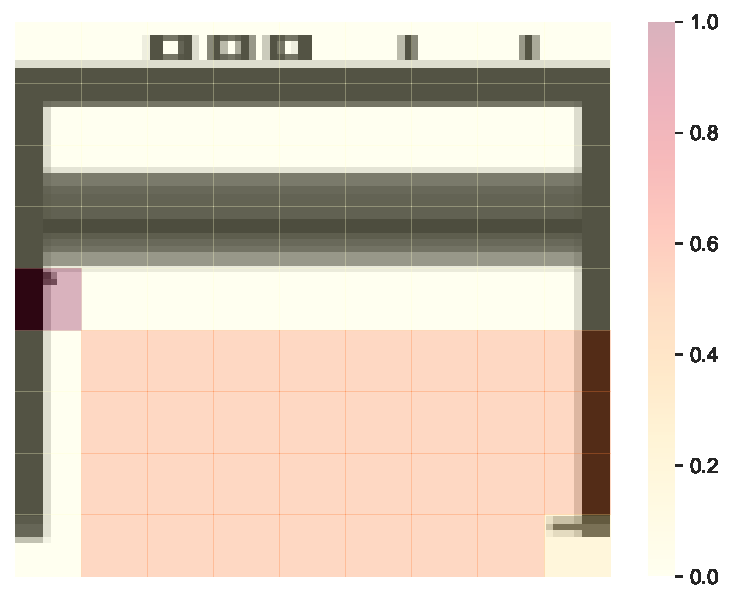
\includegraphics[width=0.65\textwidth]{plots/heatmaps/breakout_heatmap_before_reward.pdf}
    \caption{Screenshot directly before the frame hits the tiles and a reward is given. Darker areas are areas with more influence on the decision. The ball is in the darkest square.}
    \label{fig:heatmap_before_reward}
\end{figure}

\Cref{fig:heatmap_before_reward} shows the last frame before the agent gets a reward. The darker red colored areas are the areas the Interpretable CNN deems the most important for the decision. The ball is in the darkest colored square. This indicates that the Interpretable CNN learned a representation of the ball.

The same frame is shown in \Cref{fig:heatmap_before_reward_comparison}, but four different heatmaps were created based on four different snapshots taken during the training of a model. The upper left was created before training; at this point the models weights were initialized randomly and hence the heatmap was random. After 1 million frames, the heatmap looks already similar to the heatmap after 3 million frames.

\begin{figure}[ht!]
    \centering
    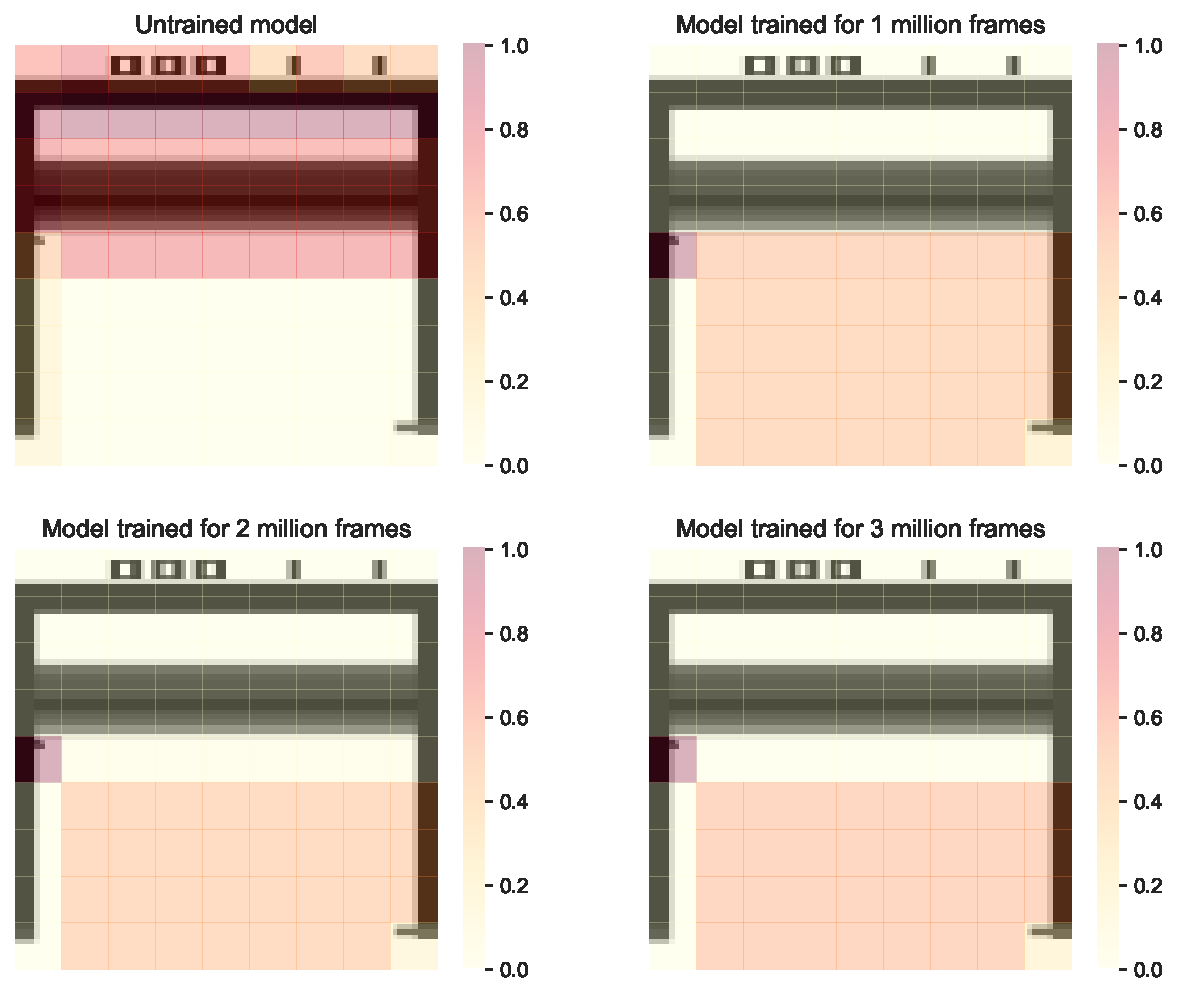
\includegraphics[width=0.9\textwidth]{plots/heatmaps/breakout_heatmap_training_comparison_before_reward.pdf}
    \caption{Screenshot directly before the frame hits the tiles and a reward is given. The dark areas are randomly spread out before training, but quickly become more expressive.}
    \label{fig:heatmap_before_reward_comparison}
\end{figure}

\begin{figure}[ht!]
    \centering
    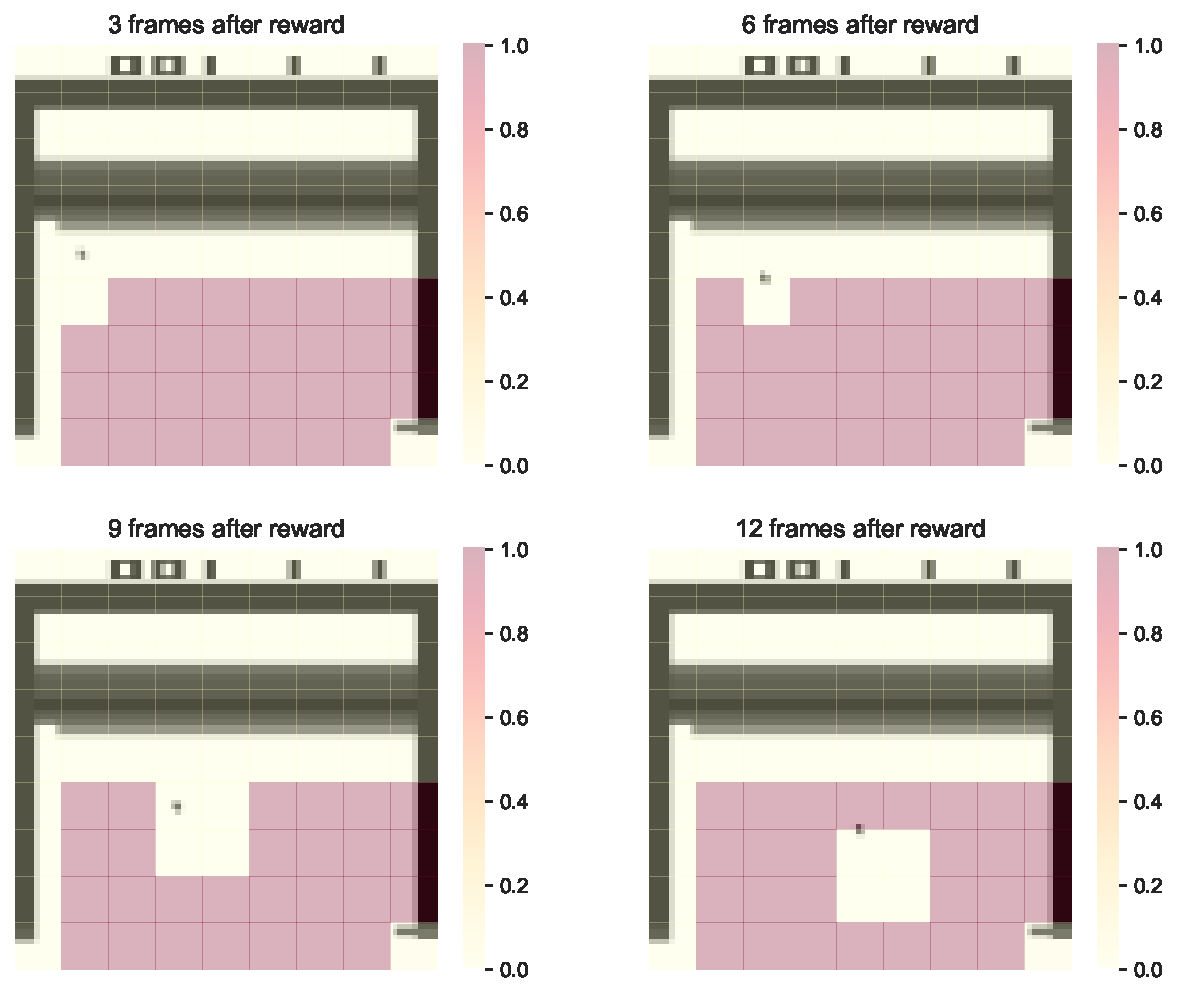
\includegraphics[width=0.9\textwidth]{plots/heatmaps/breakout_heatmap_temporal_comparison_after_reward.pdf}
    \caption{Screenshots taken several frames after the reward was given. The ball is encircled, indicating that the Interpretable CNN learned to locate the ball.}
    \label{fig:heatmap_after_reward_comparison}
\end{figure}

The ball bounces back to the player after the reward. \Cref{fig:heatmap_after_reward_comparison} shows how the Interpretable CNN has learned to locate the ball. The activation at the position of the ball is very low, but the activation around the ball is high, leading to a circle around the ball.


\FloatBarrier
\section{Individual Models}

\begin{figure}[ht!]
    \centering
    \makebox[0pt]{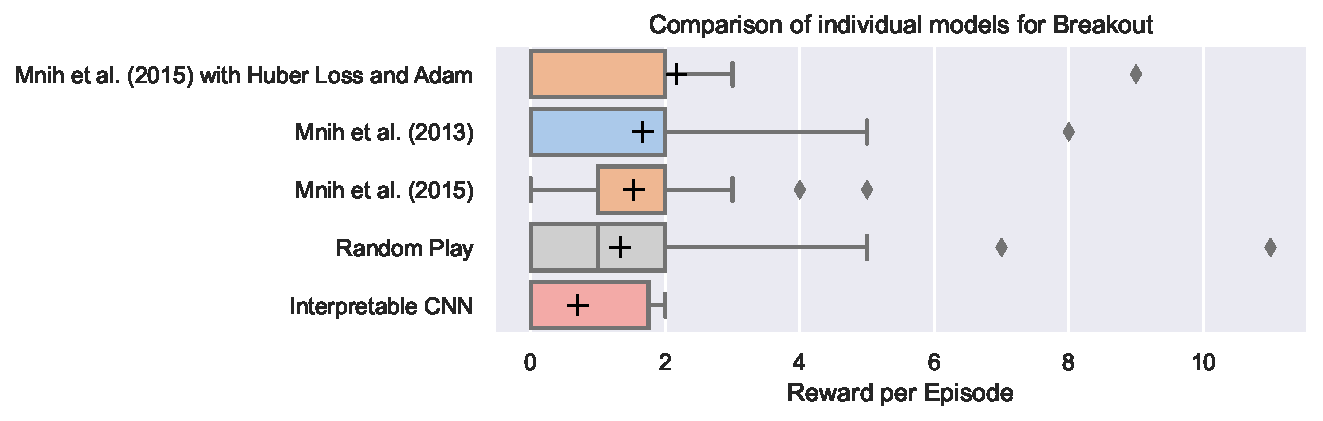
\includegraphics[width=\textwidth]{plots/reward_distribution_breakout_individual_models.pdf}}

    \makebox[0pt]{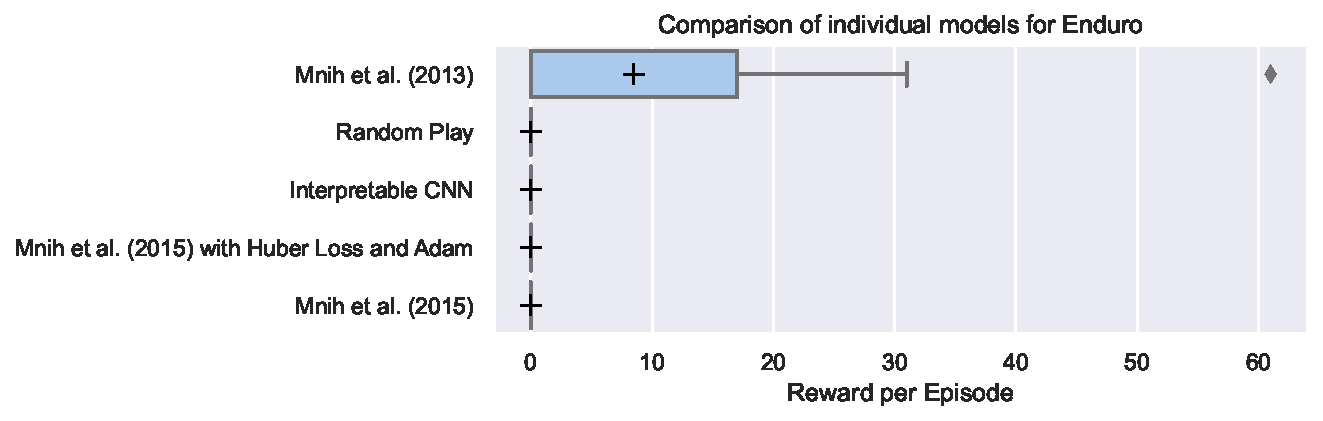
\includegraphics[width=\textwidth]{plots/reward_distribution_enduro_individual_models.pdf}}

	\makebox[0pt]{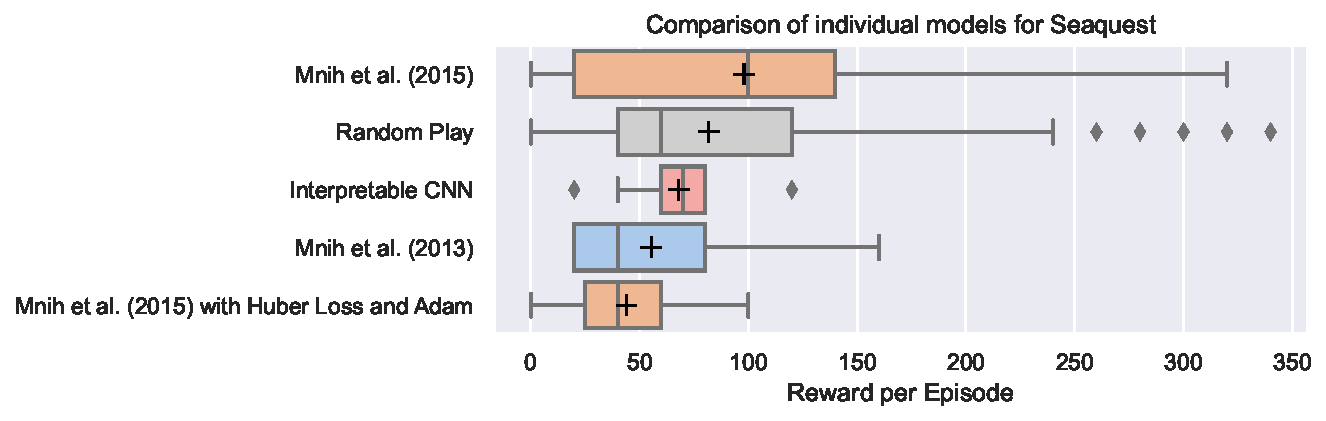
\includegraphics[width=\textwidth]{plots/reward_distribution_seaquest_individual_models.pdf}}
    \caption{Performance of individual models on Breakout, Enduro, and Seaquest.}
    \label{fig:res:individual_models}
\end{figure}

\Cref{fig:res:individual_models} shows the performance of individual models. All of the individual models, except for the Interpretable CNN, performed better than random play on Breakout. Interpretable CNN performs worse than the others, as sees only one frame (instead of four) making it impossible to learn the movement of the ball.

Only the model architecture by \textcite{mnih_playing_2013} achieved a score higher than 0 on Enduro. Enduro is a racing game where the player has to stay on the button for driving and steer to overtake cars. The DRL algorithm starts out playing random, but random play almost never leads to a long enough repetition of pressing the button to accelerate, hence only seldom receiving a reward signal from which the model can learn. That the model architecture by \textcite{mnih_playing_2013} could be a product of better random play, but also of the model architecture being smaller and learning faster from sparse reward. The results of \textcite{mnih_playing_2013,mnih_human-level_2015} tained for much longer, but also achieved much better results on Enduro. Running the DRL algorithm for longer could lead to more rewards and therefore better performance. 

On Seaquest, the model architecture by \textcite{mnih_human-level_2015} performed the best, but the same architecture but trained using Huber loss and Adam optimizer performed the worst. While Huber loss and Adam optimizer improved the performance for Breakout, they did not help for Seaquest. \textcite{mnih_playing_2013} reported that the DQN performance on Seaquest was much worse compared to humans, so it is no surprise that the models trained in this project performed worse compared to random play in Seaquest than compared to random play in other games.


\section{Ensembles}
\begin{figure}[ht!]
    \centering
    \makebox[0pt]{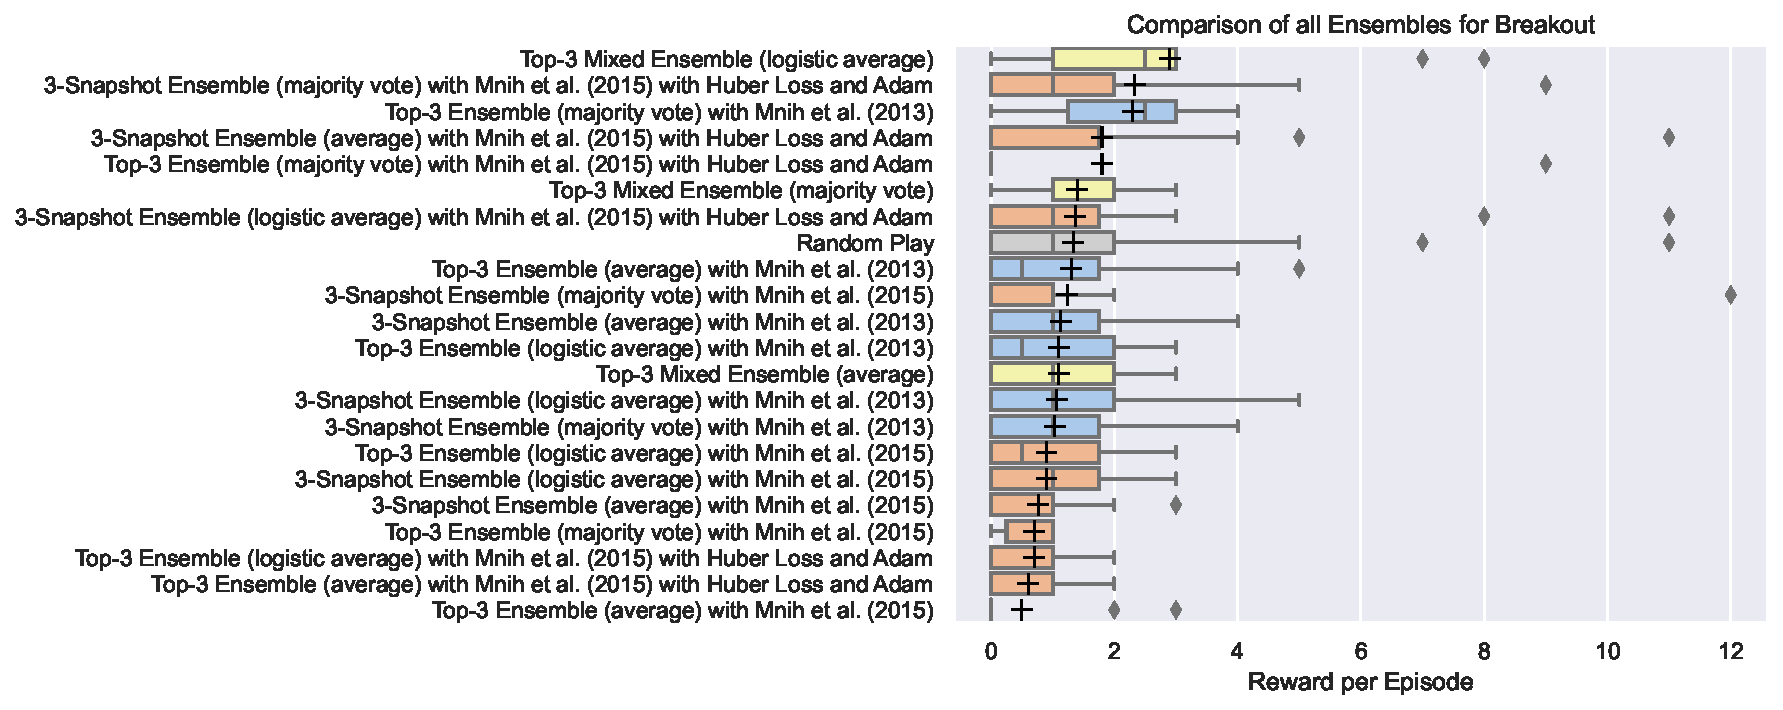
\includegraphics[width=\textwidth]{plots/reward_distribution_breakout_ensembles.pdf}}

    \makebox[0pt]{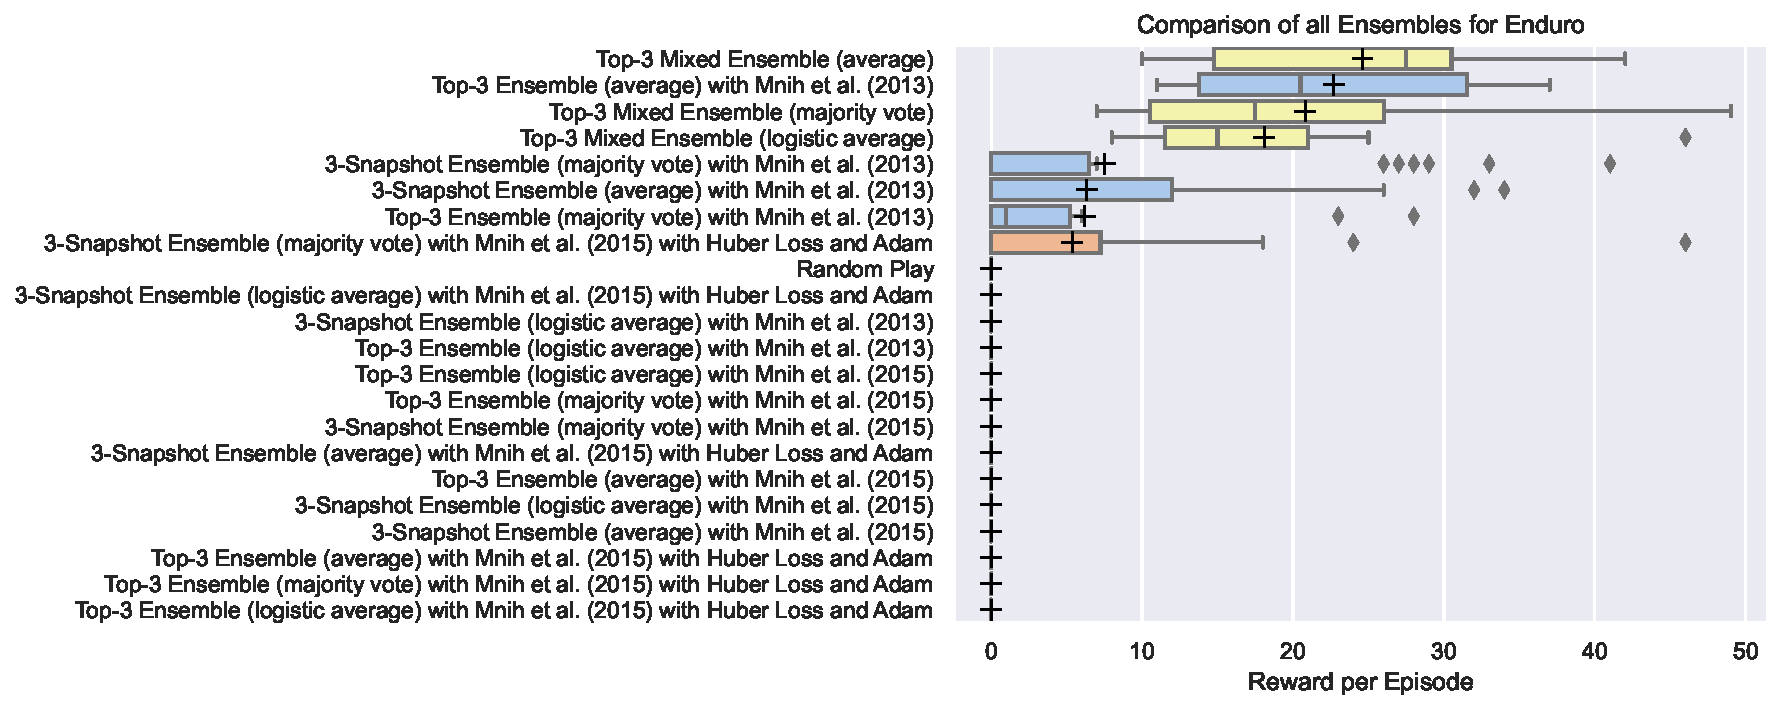
\includegraphics[width=\textwidth]{plots/reward_distribution_enduro_ensembles.pdf}}

	\makebox[0pt]{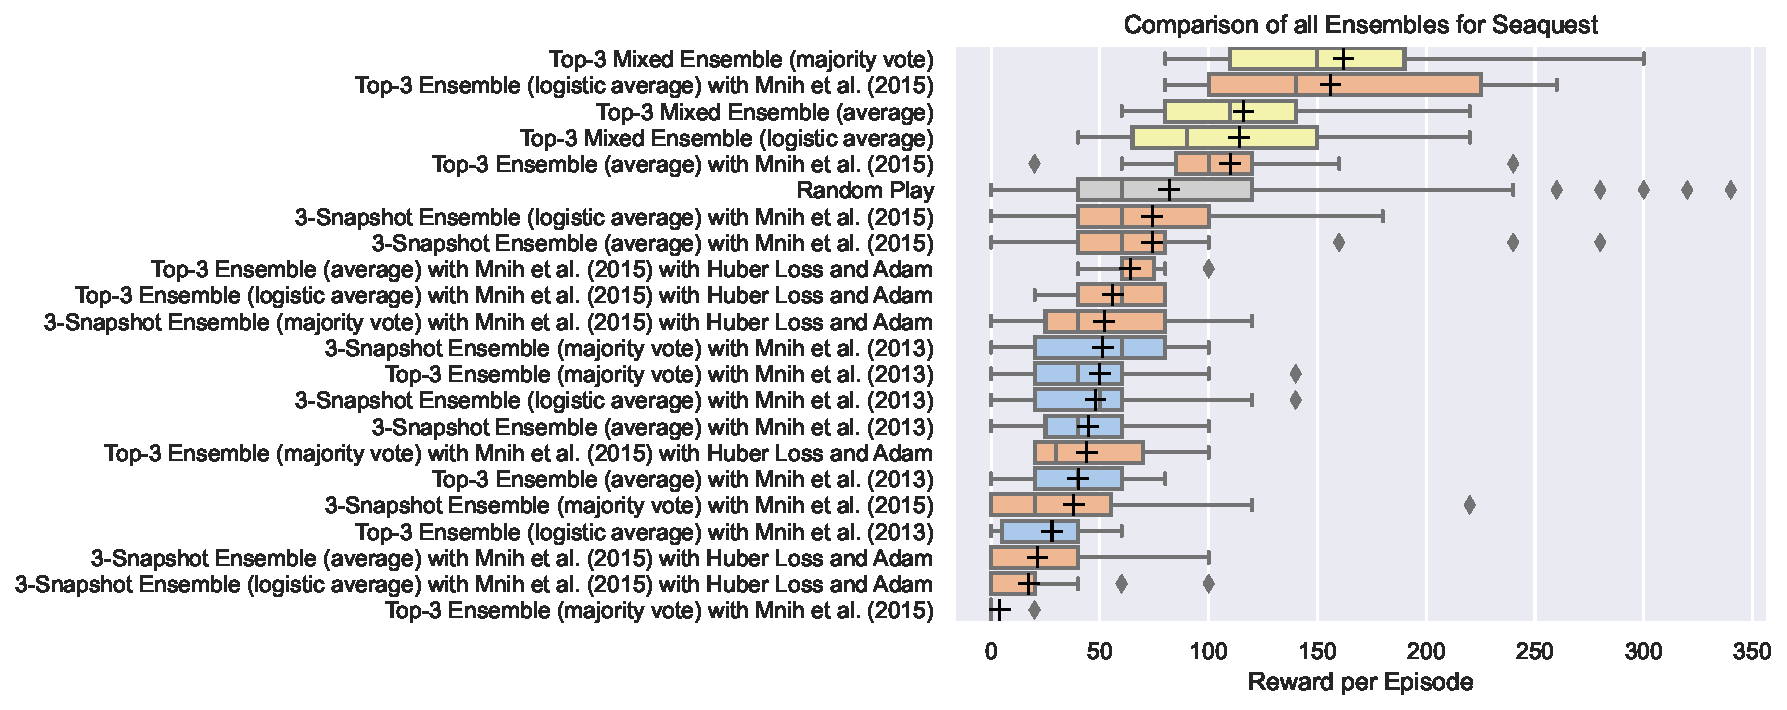
\includegraphics[width=\textwidth]{plots/reward_distribution_seaquest_ensembles.pdf}}
    \caption{Performance of Ensembles on Breakout, Enduro, and Seaquest.}
    \label{fig:res:ensembles_only}
\end{figure}

In general, the mixed Ensembles (colored yellow in \Cref{fig:res:ensembles_only}) that combine multiple different architectures seem to perform better than other Ensembles. Even though the architecture by \textcite{mnih_playing_2013} was the only individual achieving a score higher than 0 on Enduro, the mixed Ensemble of the architecture that involves all three architectures performed better than most of the Ensembles only containing models of the architecture by \textcite{mnih_playing_2013}. Interestingly, the Ensemble of 3 Snapshots of the model architecture by \textcite{mnih_human-level_2015} trained using Huber loss and Adam optimizer achieved scores higher than 0 in Enduro, even though the individual models of the same architecture did not achieve a score higher than 0.

Based on this limited data, there cannot be given a clear answer which of the ensemble methods is the best one for DRL on Atari games. The Wilcoxon pairwise significance test ($\alpha$ = 0.05) resulted in no significant difference between the different ensembles. Training the models on more different games could reveal if any of the Ensembles is superior to the others.


\section{Soups}
\begin{figure}[ht!]
    \centering
    \makebox[0pt]{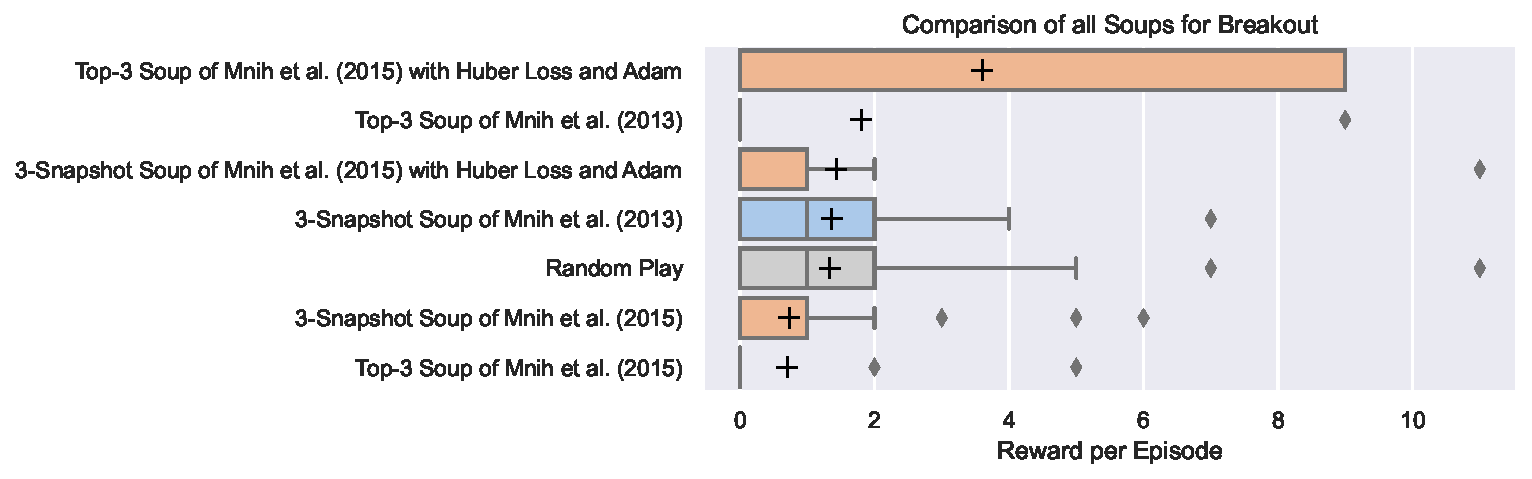
\includegraphics[width=\textwidth]{plots/reward_distribution_breakout_soups.pdf}}

	\makebox[0pt]{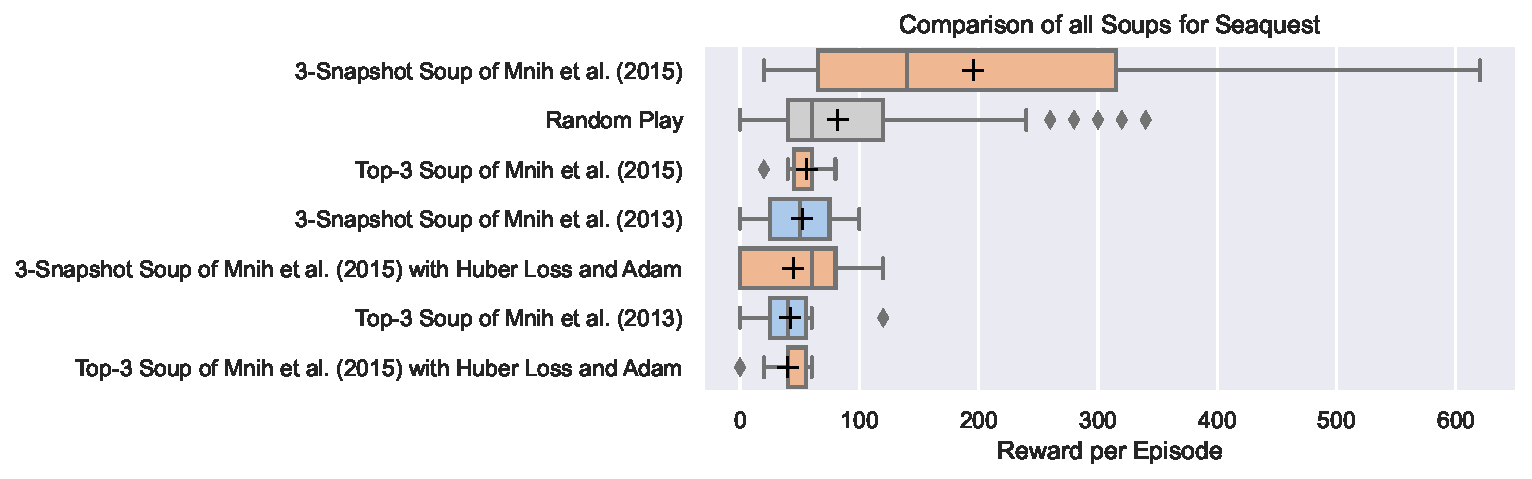
\includegraphics[width=\textwidth]{plots/reward_distribution_seaquest_soups.pdf}}
    \caption{Performance of Soup models on Breakout, Enduro, and Seaquest. (None of the Soups achieved a score higher than 0 on Enduro, hence the plot for Enduro is omitted.)}
    \label{fig:res:soups_only}
\end{figure}

None of the Soup models achieved a score higher than 0 on Enduro, hence the plot for Enduro is omitted in \Cref{fig:res:soups_only}. There seems to be no difference in performance in the Soups created from three different models of the same architecture and the Soups created from three snapshots of the same model. This is surprising: Soups take the average of the weights of the ingredient models, hence I expected the new weigths to have higher quality if they stem from the same learning procedure (snapshot Soups) and are already more similar before the averaging. The Wilcoxon pairwise significance test ($\alpha$ = 0.05) resulted in no significant difference between the different soups.


\FloatBarrier
\section{Overview}
\begin{figure}[ht!]
    \centering
    \makebox[0pt]{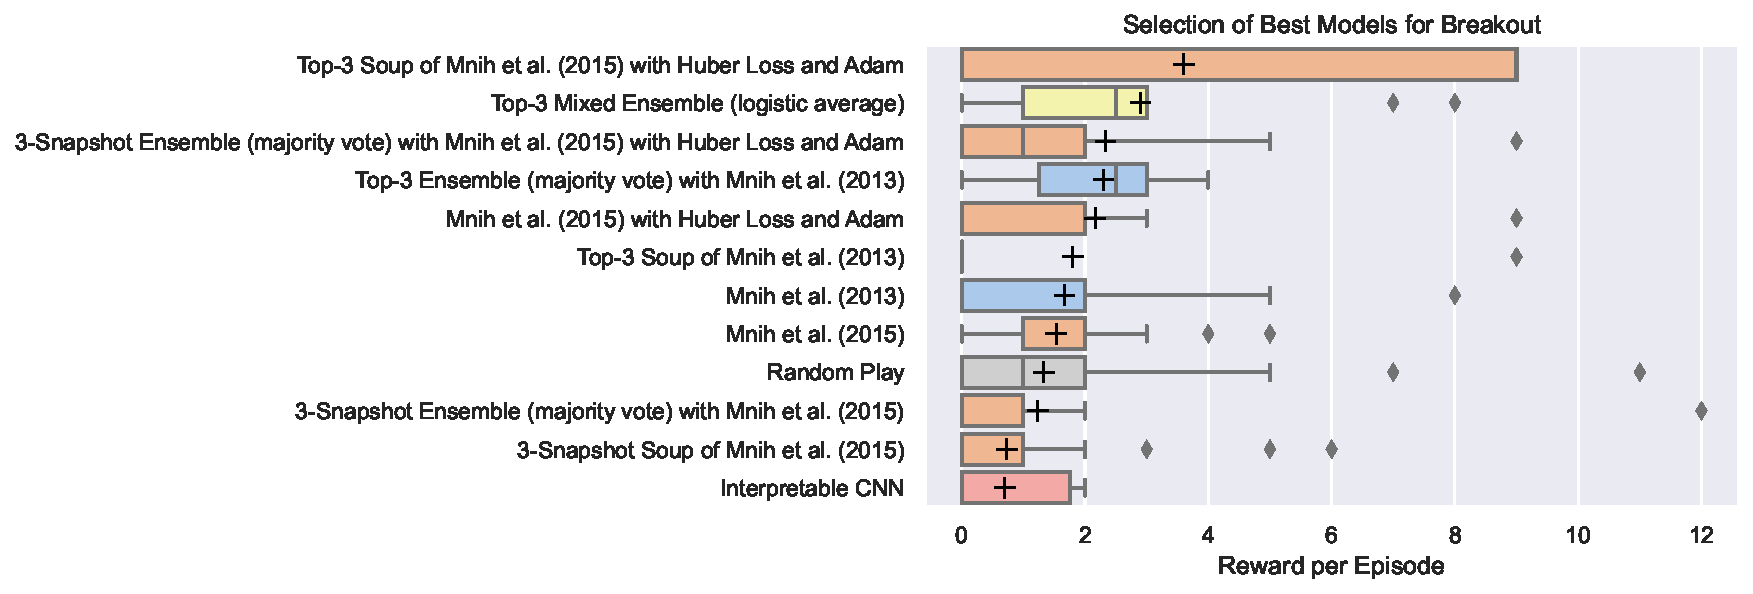
\includegraphics[width=1.1\textwidth]{plots/reward_distribution_breakout_mean_filtered.pdf}}
    
    \makebox[0pt]{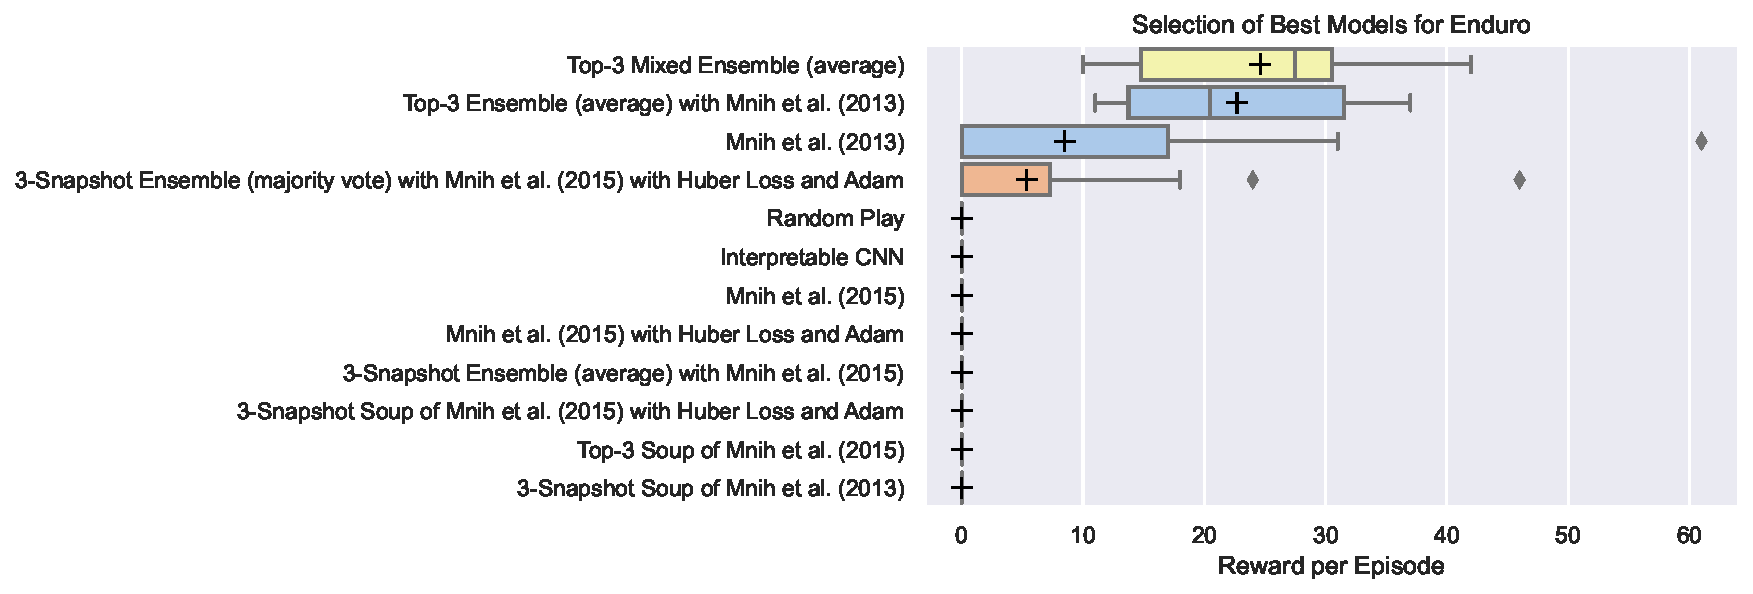
\includegraphics[width=1.1\textwidth]{plots/reward_distribution_enduro_mean_filtered.pdf}}
    
    \makebox[0pt]{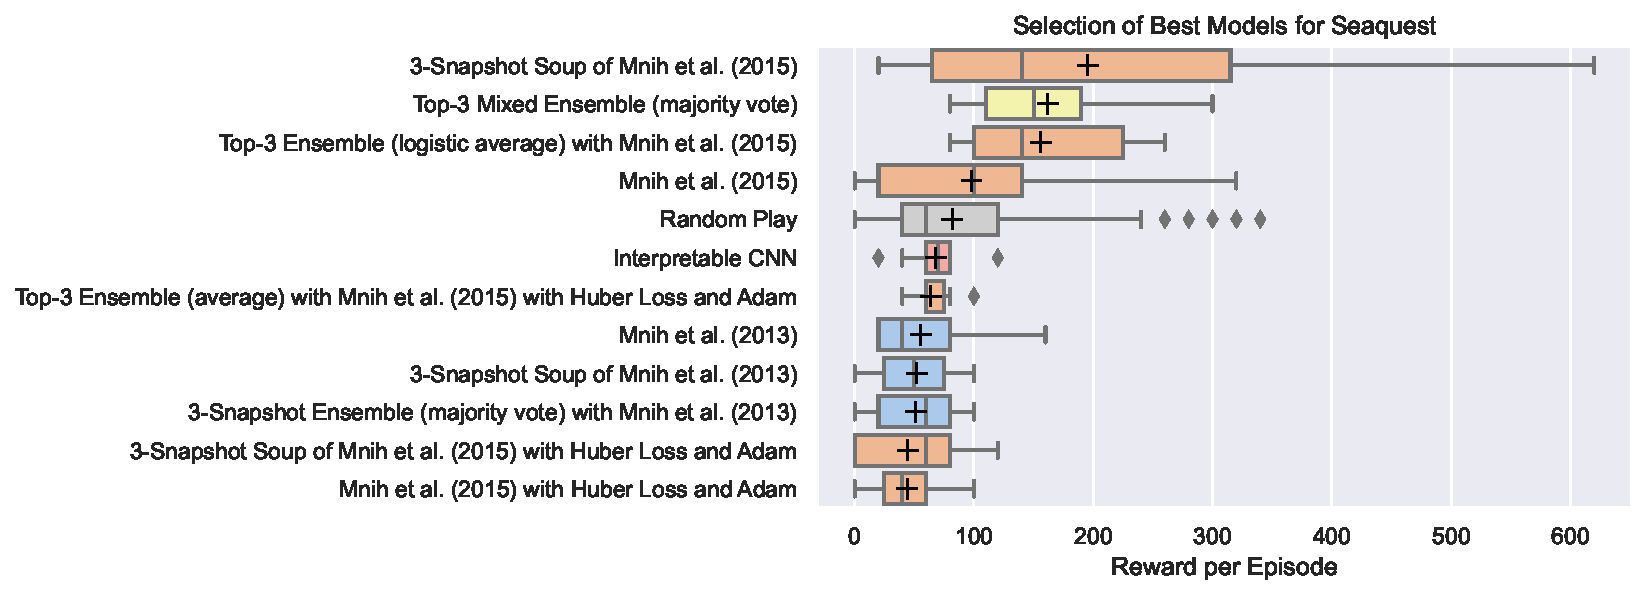
\includegraphics[width=1.1\textwidth]{plots/reward_distribution_seaquest_mean_filtered.pdf}}
    \caption{Best performing individual models, Ensembles, and Soups. The best performing models of each domain for each model architecture were selected.}
    \label{fig:res:best_models}
\end{figure}

\begin{figure}[ht!]
    \centering
	\makebox[0pt]{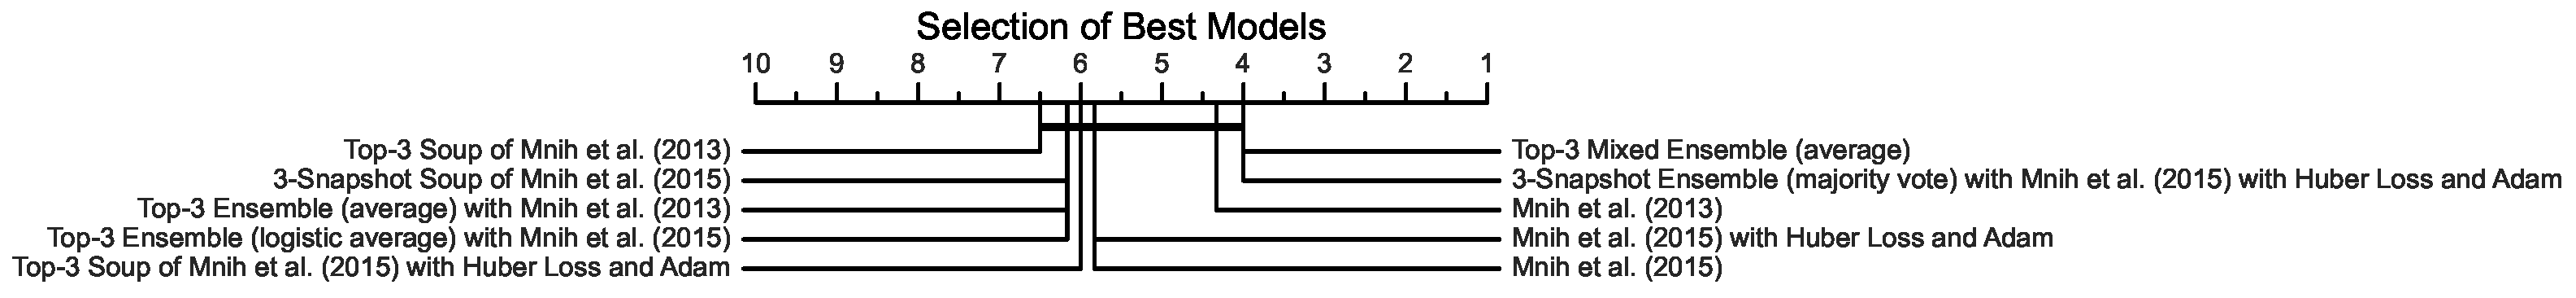
\includegraphics[width=1.2\textwidth]{cdd/cdd_selection_of_best_models.pdf}}

	\makebox[0pt]{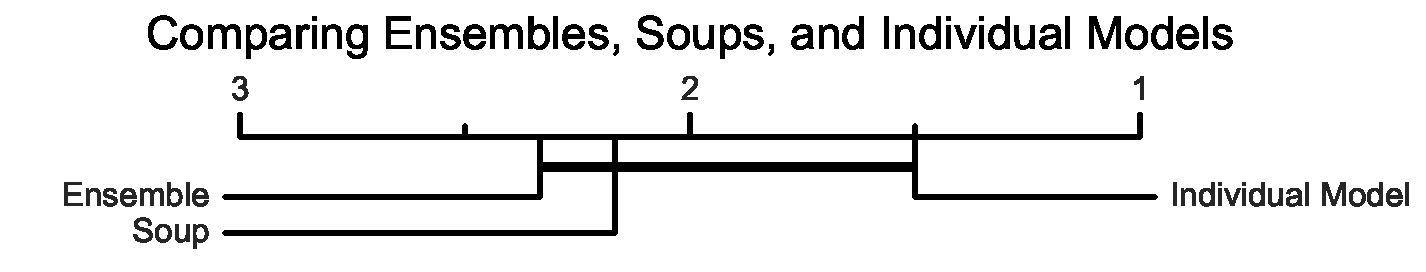
\includegraphics[width=.8\textwidth]{cdd/cdd_Ensembles_vs_Soups_vs_Individual_Models.pdf}}
    \caption{\textit{Top}: Critical Difference Diagram comparing a selection of the best performing models. No significant differences were found. \textit{Bottom}: Comparing the overall performance of Ensembles, Soups, and individual models. No significant differences were found.}
    \label{fig:cdd}
\end{figure}

This section aims to answer the question if Ensembles and Soups generelly achieve better results than single models in the context of DRL on Atari 2600 games. As \Cref{fig:res:best_models} shows, Ensembles and Soups occupy the majority of the top ranks, but also the majority of the bottom ranks. Only the mixed Ensembles containing models with different architectures achieve top performance consistently. 

The Critical Difference Diagram in \Cref{fig:cdd} shows that there is no significant difference between the best performing models of each domain. It also shows, that the comparison of all Ensembles with all Soups and all individual models does not reveal a significant difference.


\FloatBarrier
\chapter{Conclusion}

The results of this project do not support the hypothesis that Ensembles and Soups achieve better results than single models in the context of DRL on Atari 2600 games. Nonetheless, the results of this project are not conclusive, as the number of models trained is small, the models were only trained for 3 million frames, and only three games were used. 

- Does not give Information about frameworks like SUNRISE

- Fix problem with sparse rewards by integrating more time steps in future reward calculation


- Select more "easier" games
